\chapter{Control Systems}
\label{ch:control-systems}
\section{Overview}
\newcommand{\itc}{I$^2$C}
The main goal of building the software systems around the pod, was creating a redundant yet lightweight and fast solution that would allow for safe communications with the vehicle and ensure complete control throughout pod launch.\\

The Software-system is built upon the Master-Slave design model to allow for maximum redundancy and safety at all times. The design is based on three components: Embedded-systems (Controls/Sensors Hub), Communication-systems (Master), and the Control-panel. 
Embedded-systems is responsible for all of the pod's internal interactions with the sensors and various health checks. 
Communication-systems is responsible for the complete pod control and has the ability to safely shut down the pod in case of an emergency. It is also responsible for the transportation of information from the vehicle to the control-panel to allow for live data visualization and remote control of the pod. 
Front-end is responsible for displaying all of the pod's vital readings and providing a control interface while the pod is in the tube. All code written for the software system of the pod is available for public access at \href{https://github.com/teamwaterloop}{Waterloop's GitHub Page} under MIT license.

\subsection{System Overview}
Two main design decisions of the Goose III's computational design are the parallelism of launch script execution and the Master-slave design. Waterloop has defined two clear computational layers - Master-Machines and Hubs. Master-machines are responsible for the complete control of the pod and the transfer of data from Hubs to the Control-Panel. While Control-panel provides with various control of the pod during the run, the entire launch script will be stored and executed by the Master Machines. By transferring launch script execution to on-board machines, network (WI-FI network provided by SpaceX for pod communications) inconsistencies are completely eliminated.

\begin{itemize}
    \item With \textbf{Master-Slave design}, there is a clear distribution of processing requirements for each compute machine, which allows for two layers of design. Having a clear distinction allows for a powerful abstraction of all the computing operations that must be performed on the pod, which makes the system highly scalable and easier to maintain.
    \item With \textbf{parallel execution} by the three Master-machines, in the case that an active machine comes offline for an unforeseen reason, the switch to the next machine is instantaneous. All three machines will be synced in their states described in the \reffig{fig:pod-state-diag}, where one Master-machine is active and the other two are in an idle mode, but maintain the same state as the Master-machine.
\end{itemize}

\begin{figure}
  \centering
  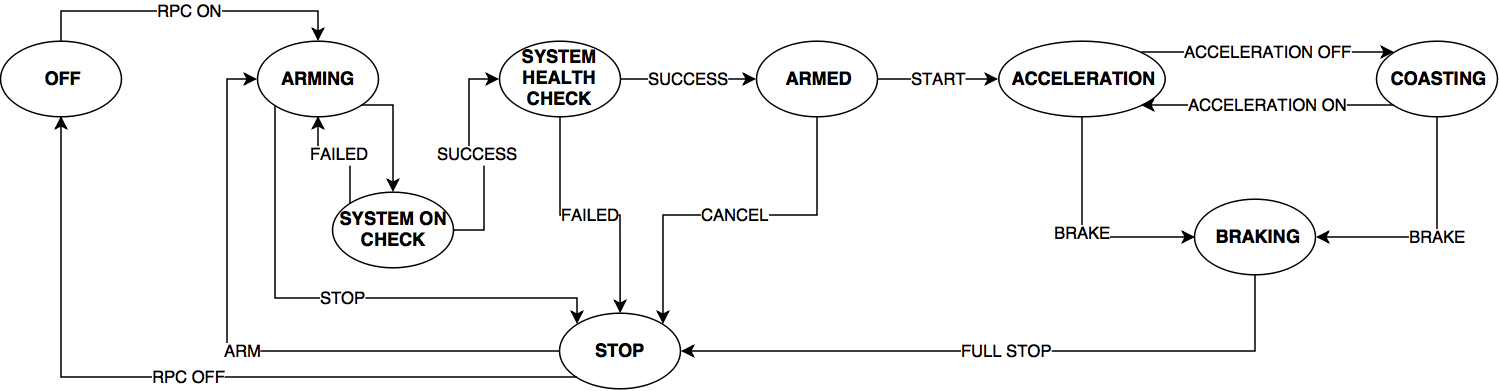
\includegraphics[width=\textwidth]{images/pod_state_diag.png}
  \caption{Pod-launch state diagram.}
  \label{fig:pod-state-diag}
\end{figure}

Based on \reffig{fig:software-diagram}, the entire system will incorporate 35 sensors, an ESC and a BMS, that will allow for a complete control over the pod and a live stream of data from all sensors.
% > 35 
% finalize # of sensors

\begin{figure}
  \centering
  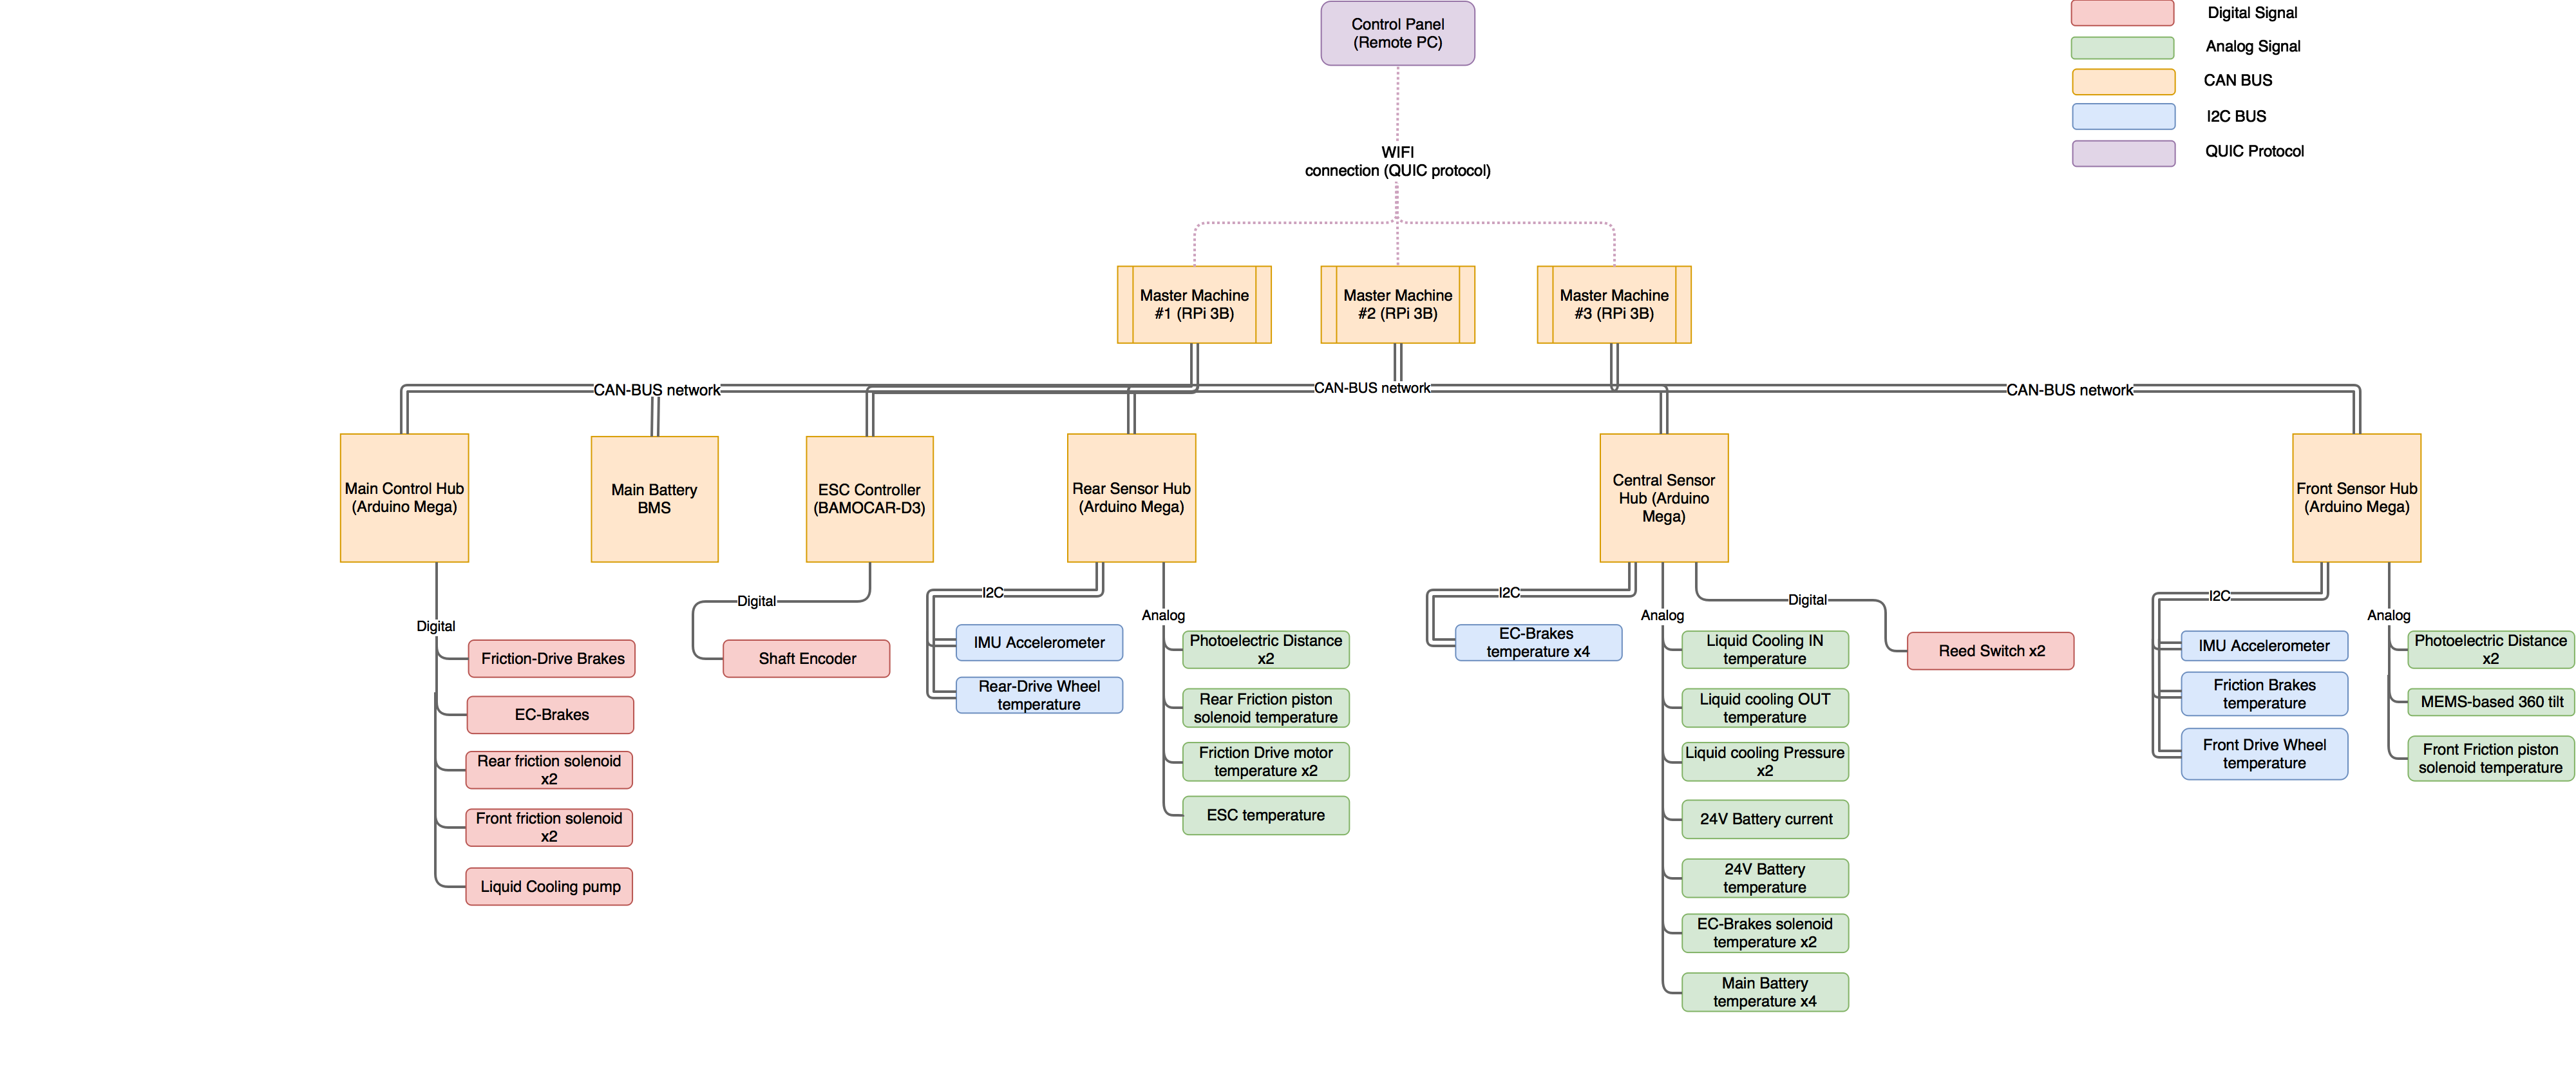
\includegraphics[width=\textwidth]{images/pod_comp_arch.png}
  \caption{Goose 3 software architecture diagram}
  \label{fig:software-diagram}
\end{figure}

\section{Communication System}
Three major design decisions had to be made in order to develop a powerful, yet lightweight and fast communication pipeline to transfer packets from the low-level Hubs to a high-level Control-Panel.
\begin{itemize}
    \item Selecting the best packet type to create a fast and reliable communication channel; packet loss vs. packet speed trade-off
    \item Master-Slave design to allow for a powerful, yet modular and scalable system
    \item Developing an abstract package structure that allows for transfer of data from Slave to Master-machines with minimal overhead cost
\end{itemize}
We have decided to use a custom packet structure to transfer data at minimum overhead costs between Slave and Master-machines and a Golang server with QUIC packet streams to transmit data to the Control-Panel wirelessly

\subsection{Server and Network Protocols}
\label{subsec:comm-protocols}
\textbf{Golang vs. Node.js Server:} Go allows for language level concurrency with Go routines and has faster raw performance than our previous event-based Node.js server, decreasing overall latency. The server acts as a 'middle-man' communication channel between the low level Embedded-systems hubs and the high level Control-panel.\\

\noindent\textbf{TCP vs. QUIC Streams:} QUIC has built-in data reliability checks to eliminate packet loss and establishes connections much faster than TCP by removing the slow handshake process\footnote{\url{https://www.chromium.org/quic}}.
It is built on top of UDP and allows for multiplexing to provide extremely fast data transmission rates with minimal latency. After testing packet transmission speeds over a fairly stable wireless connection using TCP, UDP and QUIC streams, our results summarized in \reffig{fig:tcp_vs_quic} showed that multiplexed QUIC performed significantly faster (by up to approximately 20x depending on number of streams used) compared to both TCP and UDP.\\
\begin{figure}
\centering
\begin{subfigure}{0.7\textwidth}
    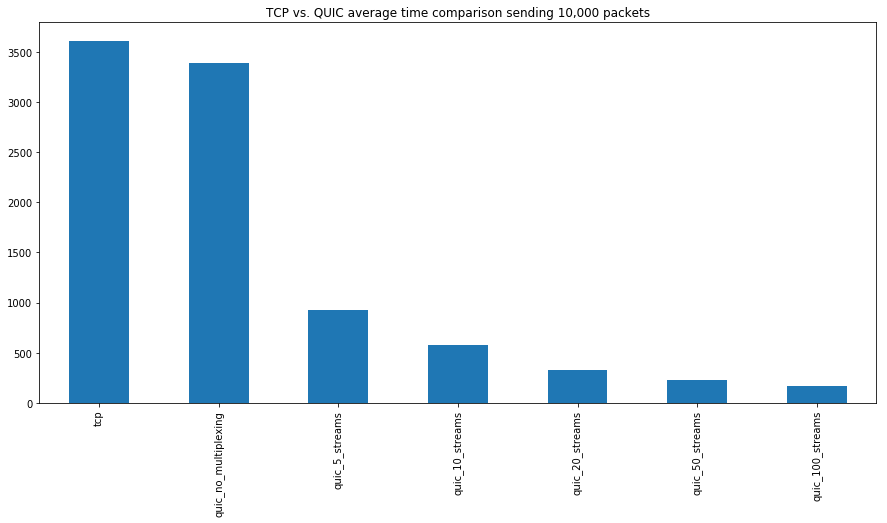
\includegraphics[width=\linewidth]{images/tcp-quic-bar-graph.png}
    \caption{Histogram}
\end{subfigure}
\begin{subfigure}{0.7\textwidth}
  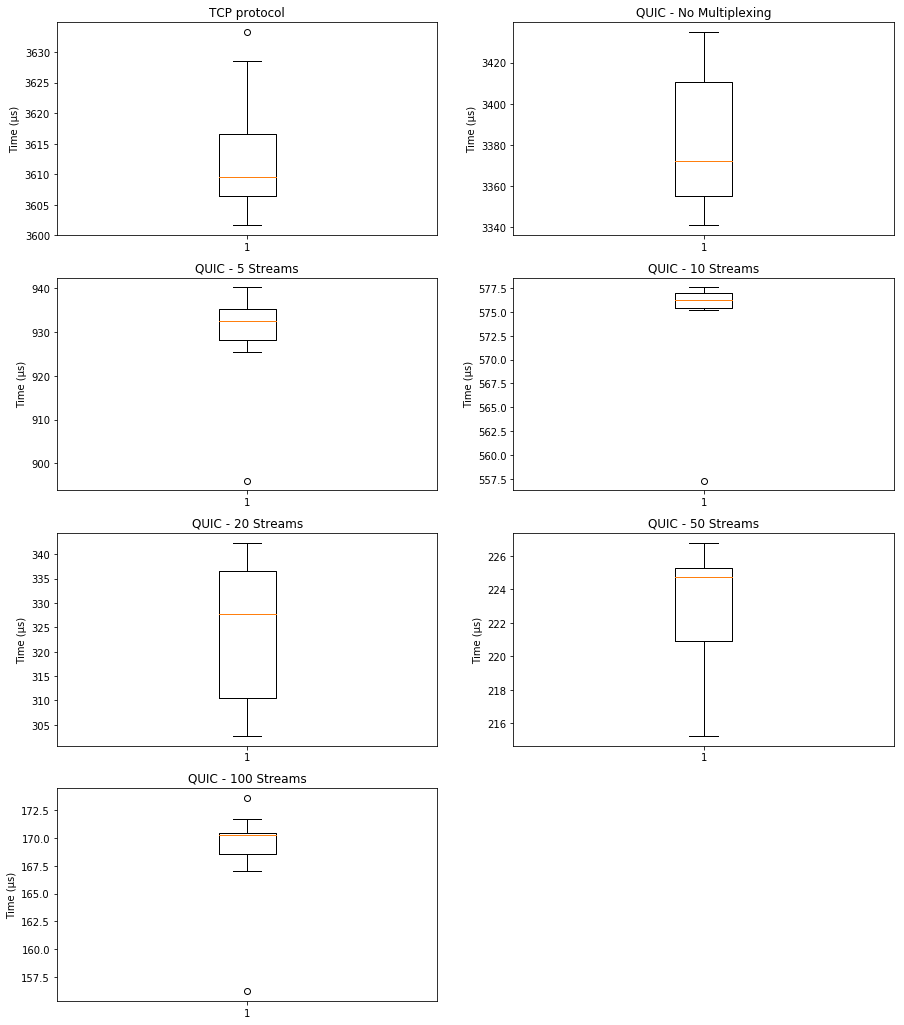
\includegraphics[width=\linewidth]{images/streams-box-plots.png}
  \caption{Box Plots}
\end{subfigure}
	\caption{TCP vs. QUIC w/ no multiplexing vs. QUIC w/ multiplexing}
  \label{fig:tcp_vs_quic}
\end{figure}
As a result of a series of tests (\reffig{fig:tcp_vs_quic}), QUIC streams will be used to transmit control commands from the high level Control-panel (front-end client) and raw data back (from front-end client) to the on-board control elements. Multiple input and output streams can be opened across the server and client which allows for the simultaneous transmission of data packets from different sensors. The convention for all communications will be to use individual ordered output streams to transmit important sensor data packets that require ordered processing and individual input streams for all control packets coming in from the Control-panel.\\

\noindent\textbf{CANBUS:} Raw data packaged into Waterloop's custom defined packet structure will be transmitted through a CAN-bus network for communication between low-level Hubs and the communication server. As an alternative, \itc with all Hubs and Masters connected in parallel has been considered to be used instead of the CAN-BUS network. Two main factors have been used to select CAN-BUS over an \itc network:
\begin{itemize}
	\item Distance limitation of the \itc network. Usually used for internal PCB components, not for vehicle long communication.
    \item Speed limitation of the \itc network. CAN-BUS can allow up to \SI{1}{Mbps} packet transfer speed on much longer distances\footnote{\url{http://www.can-wiki.info/doku.php}}.
\end{itemize}

\paragraph{CAN-BUS Protocol Description}
CAN is a protocol that was designed for vehicle controller commutations to transmit information in a network without a host computer. It is a message based protocol with built-in priority and error checking. The priority allows for nodes to send higher priority messages, which places them higher in the message priority queue. Error checking allows for frames to check for losses and discard if they contain errors.

\subsection{Communication-System redundancy measures}
\qquad\textbf{Parallel Master-Machines} In order to ensure instantaneous recovery options, Waterloop will run three identical Master-Machines, with one being active and the others inactive. The active machine will be responsible for execution of bidirectional communication and execution of all control commands, as well as the pod-launch script. In the mean time, the inactive machine will stay up to date with the state of the active machine. In case of the failure of the active machine, measures such as heartbeat will allow for instant detection of device failure and and a switch to one of the idle machines into an active state. Control-Panel, using heart-beat as well, will detect the change of active machine and will adjust by restarting the failed Master-machine and putting it into inactive state once the reboot is complete.\\

\textbf{Distributed System} Communication-system's distributed system will be achieved by running three Raspberry Pi controllers at the same time using a Docker Swarm. This will use the Raft consensus algorithm with an internal distributed state store to determine validity of data for each node and verify consistent data across all three controllers. The nodes will communicate through \itc.\\
    The Docker Swarm allows for two types of nodes, the manager node and worker node. Manager nodes distribute tasks among other worker nodes, and send data to the client through the communication protocols described in \refsubsec{subsec:comm-protocols}. Worker nodes perform the same tasks as other workers to reach consensus and can have tasks distributed among them.\\
    Initially at runtime, the pod will have a single manager node and two worker nodes running concurrently, where in the case of a manager failure, one of the worker nodes will be promoted to a manager.\\
    Controller failure will be monitored through a heartbeat managed by Docker which uses a small timeout for nodes to respond.
    
\section{Control Packet Format}
    \subsection{JSON structure}
    \label{subsec:json}
    All communications between on-board Master-machines and Control-panel are JSON packets serialized from Go structures in the following format:
	\begin{minted}{go}
type CommPacketJson struct {
    Time int64      `json:"time"`
    Type string     `json:"type"`
    Name string     `json:"name"`
    Data []float32  `json:"data"`
}
    \end{minted}
    \begin{table}[H]
        \centering
        \begin{tabular}{@{}lp{4in}l@{}} \toprule
            Property & Description & Example\\ \midrule
            \texttt{time}
            & Time of packet creation, in milliseconds since Unix epoch & \tabxmintinline{json}{1513452619442}\\
            \texttt{type} & Packet type, see possible packet types & \tabxmintinline{json}{"sensor"}\\
            \texttt{name} & Specific name of packet, explicitly describing role and origin of packet (i.e. data from a specific sensor) & \tabxmintinline{json}{"accel1"}\\
            \texttt{data} & 3-tuple of float32 values representing packet data & \tabxmintinline{json}{[32.2323, 12.22, 23.11]}\\ \bottomrule
        \end{tabular}
        \caption{Description binary packet fields}
    \end{table}
    Example of a serialized JSON:
    \begin{minted}{json}
{
    "time": 1513452619442,
    "type": "sensor",
    "name": "accel",
    "data": [0.00, 0.00, 0.00]
}
    \end{minted}
    \subsection{Binary Packet Structure}
    Communication between slaves (Arduino) and on-board masters (Raspberry Pi) consists of 64-bit CAN data packets, the structure of which is described below. Packets are checked with a CRC-8 checksum $(0$x$97 = x^8 + x^5 + x^3 + x^2 + 1)$.
    \begin{table}[H]
        \centering
        \begin{tabulary}{\textwidth}{@{}LLlll@{}} \toprule
            {[0:2]} & {[3:9]} & {[10:27]} & {[28:45]} & {[46:63]}\\ \midrule
            3 bits & 7 bits & 18 bits & 18 bits & 18 bits\\
            Packet Type & Packet Name & Data value 1 & Data value 2 & Data value 3\\ 
            \\
            see \ref{par:packet-name-repr} & see \ref{par:packet-name-repr} & & see \ref{par:data-repr} \\ \bottomrule
        \end{tabulary}
        \caption{Binary packet structure breakdown}
    \end{table}
    \paragraph{Packet Type Representation}
    \label{par:packet-type-repr}
    Each packet type is represented by 3 bit encoding
    \begin{table}[H]
        \centering
        \begin{tabular}{@{}ll@{}} \toprule
            Bits & Type\\ \midrule
            000 & sensor\\
            001 & command\\
            010 & state\\
            011 & log\\ \bottomrule
        \end{tabular}
        \caption{Packet types mapped to binary representation}
    \end{table}

    \paragraph{Packet Name Representation}
    \label{par:packet-name-repr}
    Each packet name is represented by 7 bits. All of the 35 sensors on-board of the pod will be represented using the 7 bit binary codes. Having $2^7=127$ possible sensor encodings, there are more than enough combinations to cover all on-board sensors of the Goose 3 pod.

    \paragraph{Data representation}
    \label{par:data-repr}
    Data values are floats represented by 18 bits as follows:
    \begin{table}[H]
        \centering
        \begin{tabular}{@{}lll@{}} \toprule
            Sign & Exponent & Significand\\ \midrule
            1 bit & 5 bits & 12 bits\\ \bottomrule
        \end{tabular}
        \caption{Structure of 18-bit float. Significand has 13 bits of precision with 12 explicitly stored.}
    \end{table}
    This representation follows from the IEEE specifications for half and full precision floating point numbers. This allows us a max value of \texttt{65504} and a minimum positive normal of about \texttt{1.5258789e-5} with approximately 4 significant digits.
    \section{Communication Packet Types and Usage}
    Packets can be exchanged between Embedded-systems and Controls-panel depending on type. There are four main types of packets that will be used (1) Command, (2) Sensor, (3) Log and (4) State Packets.
    \subsection{Command}
    Command packets are unidirectional from Control-panel to the control elements on the pod.
\def\tabxmintinline#1#2{%
\ifx\@footnotetext\TX@trial@ftn
\detokenize{#2}%
\else
\mintinline{#1}{#2}%
\fi}
\makeatother
    \setmintedinline[json]{breaklines}
	\begin{table}[H]
        \centering
        \begin{tabular}{@{}lllp{3.8in}@{}} \toprule
            Name & Code & Value(s) & Example\\ \midrule
            Brake & \texttt{brk} & None & \tabxmintinline{json}{{"time": ..., "type": "command", "name": "brk", "data": []}}\\
            Emergency & \texttt{emg} & None & \tabxmintinline{json}{{"time": ..., "type": "command", "name": "emg", "data": []}}\\
            Speed & \texttt{spd} & \texttt{0.00 - 100.00} & \tabxmintinline{json}{{"time": ..., "type": "command", "name": "spd", "data": [100.00]}}\\
            Start Pod & \texttt{start} & None & \tabxmintinline{json}{{"time": ..., "type": "command", "name": "start", "data": []}}\\
            Stop Pod & \texttt{stop} & None & \tabxmintinline{json}{{"time": ..., "type": "command", "name": "stop", "data": []}}\\
            Health Check & \texttt{health} & None & \tabxmintinline{json}{{"time": ..., "type": "command", "name": "health", "data": []}}\\
            Coast & \texttt{coast} & None & \tabxmintinline{json}{{"time": ..., "type": "command", "name": "coast", "data": []}}\\
            Accelerate & \texttt{accel} & None & \tabxmintinline{json}{{"time": ..., "type": "command", "name": "accel", "data": []}}\\ \bottomrule
        \end{tabular}
        \caption{Control-panel to Pod command packet examples}
    \end{table}

\subsection{Sensor}
    Sensor packets are unidirectional and are sent from pod's Embedded-system to the Control-panel where all data is visualized in series of graphs.
    \begin{table}[H]
        \centering
        \begin{tabular}{@{}lllp{3.65in}@{}} \toprule
            Name & Code & Value(s) & Example \\ \midrule
            {[Sensor Name]} & \texttt{[sensor code]} & None & \tabxmintinline{json}{{"time": ..., "type": "sensor", "name": "accel", "data": [12.11, 12.34, 43.21]}} \\ \bottomrule
        \end{tabular}
        \caption{}
    \end{table}

\subsection{Log}
    Hubs and Master-machines are capable of sending Log messages that are displayed on the Control-panel and stored in Pod's non-volatile memory. The stored log messages can be accessed post-launch for launch analysis.
    \begin{table}[H]
        \centering
        \begin{tabular}{@{}lllp{3.9in}@{}} \toprule
            Name & Code & Value(s) & Example \\ \midrule
            {[Any name]} & \texttt{[any code]} & Any values & \tabxmintinline{json}{{"time": ..., "type": "log", "name": "accel", "data": [12.11, 12.34, 43.21]}} \\ \bottomrule
        \end{tabular}
        \caption{Example of Log message packet}
    \end{table}
    
\subsection{State}
    Sent from Control-panel or Embedded-systems to update state of Master-Machines
    \begin{table}[H]
        \centering
        \begin{tabular}{@{}lllp{4.25in}@{}} \toprule
            Name & Code & Value(s) & Example \\ \midrule
            Braking & \texttt{brk} & \texttt{0, 1} & \tabxmintinline{json}{{"time": ..., "type": "state", "name": "brk", "data": [1]}} \\ \bottomrule
        \end{tabular}
        \caption{Example of state packet}
    \end{table}
 
    \subsection{Data Logging and Blackbox}
    In the short-term, Generic data logging will be implemented by storing all transmitted sensor data and pod commands into JSON files onto the Raspberry Pi as a blackbox. Data from each sensor will be written to separate files to allow for future data processing and analysis of patterns.\\
    As a long-term data storage solution, Waterloop will use AWS S3 to store large amounts of data without sacrificing accessibility. For post-launch data analytics, a local Grafana UI will be built to provide quick and modular data visualization tools, thus allowing the team to debug every single pod launch.
       
        
\section{Navigation System}
Navigation system will be running on all Master-machines and will use a variety of inputs to generate a precise location of the pod inside the tube. The system will be based on two IMUs, a Shaft Encoder and a Timer. Since raw data from accelerometers has a lot of variability due to the sensitivity of sensors, the IMU outputs will be passed through a Kalman filter. In addition to a data filter, the three on-board IMUs can be used for correctness voting. Since there is an odd number of IMU sensors, a basic voting algorithm will allow for a simple consensus procedure. \reffig{fig:navigation-system} Describes the flow of data within the Navigation-system.

\begin{figure}
    \centering
    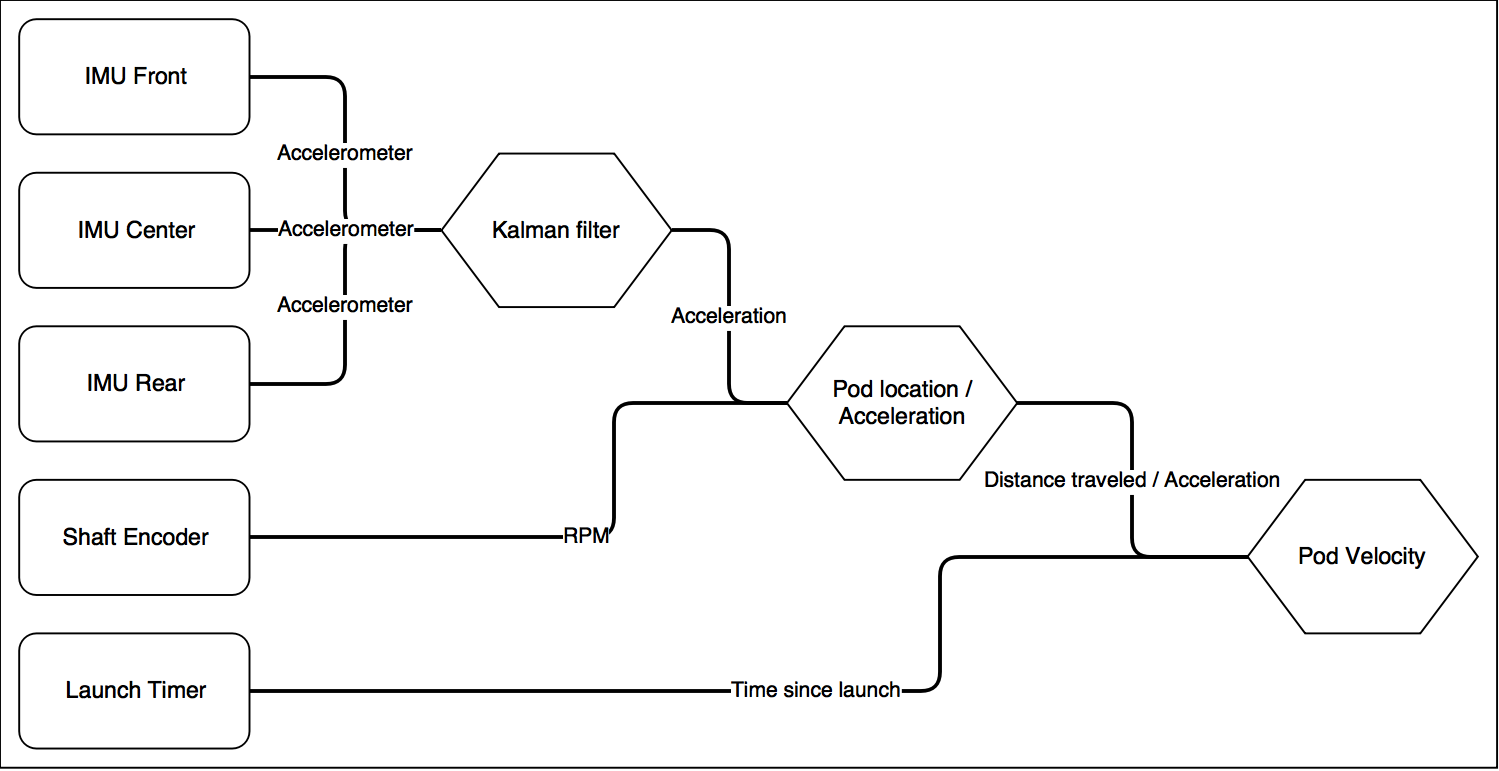
\includegraphics[width=\textwidth]{images/navigation_system.png}
    \caption{Simulation of data flow within the Navigation-system on the pod.}
    \label{fig:navigation-system}
\end{figure}

\section{Safety of Embedded \& Communication Systems}
\subsection{Pre-launch Tests}
\begin{table}[H]
	\centering
	\begin{tabular}{@{}lll@{}} \toprule
    Sub-System & Test Description & Nominal Values \\ \midrule
    Motor & Nominal Current Draw at ESC & \\
    Motor & Nominal Temperature MOTOR & \\
    Motor & Nominal Temperature ESC & \\
    Motor & Cooling pump is active, cooling pressure less than & $< \SI{14.5}{psi}$ \\
    Friction & Pressure sensor & $< \SI{250}{psi}$ \\
    Friction & Solenoid control to turn on and off & TRUE \\
    Batteries & Nominal Voltage and Current Main Battery & \\
    Batteries & Nominal Temperature Main Battery & $20 < \textrm{Temp} < 50$ \\
    Batteries & Nominal Voltage and Current 24V Battery & 24 volts \\
    Batteries & Nominal Temperature 24V Battery & $20 < \textrm{Temp} < 50$ \\
   	Batteries & Nominal Voltage from 25V to 5V step-down & 5 volts \\
    Navigation & IMUs are functional and give normal values  & \SI{0}{m/s} acceleration \\
    Navigation & Shaft Encoder at \SI{0}{rpm} and Functional & Drive Test \\
    Navigation & Tilt sensors nominal values and online & $< 10 ^\circ$ \\
    Navigation & Test Navigation system working (drive 1 meter) & Output 1 meter \\
    Navigation & ESC output is nominal & Drive Test \\
    EC-Brakes & Reed sensor state & \\
    EC-Brakes & Nominal Temperature & \\
    EC-Brakes & Solenoid Controls online & \\
    Other & Photoelectric distance is Nominal & \\ \bottomrule
    \end{tabular}
	\caption{Pre-Launch Self-Checks. Will be ran on pod before any launch. Described as System Health Check in pod state diagram \reffig{fig:pod-failure-state-diagram}}
    \label{tlb:prelaunch-tests}
\end{table}

    \subsection{Heartbeat}
    There are going to be three types of heartbeats in the system:
    \begin{itemize}
      \item Master-machine $\rightarrow$ Control-panel Heartbeat
      \item Hub $\rightarrow$ Master-machine Heartbeat
      \item Sensor $\rightarrow$ Hub Heartbeat
    \end{itemize}
    
    In case of any of the heartbeat failing, the master that is being reported to, is capable of restarting a slave i.e. triggering the watchdog procedure.
    
	\subsection{Watchdogs}
    With two types of machines used in the pod's Embedded-systems, ATMega and RPI, each one has a different approach to Watchdogs. Arduino has a built in Watchdog that can be configured and with it's non-volatile memory, a lot of the state information can be preserved and recovered after a reboot. RPI has an OS-level Watchdog as well, but having a much more complex OS to load, reboots will take longer. Exact number will be generated through a series of tests.
   
    \subsection{Single points of failure}
    By the physical nature of the CAN-BUS requiring two wires for communication and being bus based topology if a bus wire is disconnected or breaks, the nodes will lose all communications and the last sent packet will be damaged and lost. Disconnecting device from the bus will cause errors as a CAN node that doesn't receive any acknowledgement for a packet it has sent, will keep trying to send it indefinitely, hence clogging the bus pipeline. Both cases will trigger a failure mode as heartbeats will not be received stopping the pod. Thus, even with these failure cases the pod will still be able to come to a controlled stop.
    
    \subsection {Failure scenarios and state diagram}
  In the event of pod failures, the control system will respond accordingly to ensure no harm is caused to the pod, the team, the test track, or the environment. If a system fails, the pod is designed to ensure it is just as safe as when it was operating correctly.\\
  The following table below lists the failure modes and effects according to specific failure scenarios. The software failure scenarios include, but are not limited to: the main battery, embedded system, braking, navigation, friction drive, and sensors.
  The software failure state diagram \reffig{fig:pod-failure-state-diagram} shows the behaviour and flow of the control systems. In addition, \reftab{tlb:fail-table} shows all of the possible failure scenarios and according software actions that are taken as a consequence.\\
  
\begin{table}[p]
\centering
\begin{tabular}{@{}p{3cm}p{13cm}@{}}
\toprule 
 Source & Action\\
\midrule
Main Battery dies or fails & EC brakes engage based on circuit design, provide power to friction brakes if speed is less than \SI{10}{m/s}\\
% \hline
Server side power wire is down& Case 1: One server dies, switch to the next server; Case 2: All servers die, Embedded loses heartbeat\\
% \hline
Embedded subsystem dies& Active server will ground the pod\\
% \hline
Friction subsystem dies& Activate braking, cut off power to motor\\
% \hline 
Braking subsystem dies& Keep navigation active; Keep safety mechanisms on; Shut down other systems\\
% \hline
Navigation subsystem dies& Brakes: Keep braking; Acceleration: Cut off acceleration, activate EC/friction brakes; If speed is greater than 10 m/s, do not activate friction\\
% \hline 
Brakes overheat& Braking: Keep braking (Friction and EC brakes); Acceleration: Cut off acceleration, activate EC/Friction brakes\\
% \hline
24V battery dies or fails&Case 1: 1 battery dies: Brakes engage; Provide power to friction drive if speed is less than 10 m/s; Case 2: both batteries die:  Lose all 3 servers, Embedded loses heartbeat; Brakes engage\\
% \hline
Friction drive slips on the rail&Use a filter if there is a spike (non-linear slope); If friction drive slips for less than 0.5 seconds, cut friction, stop accelerating; If 0.5 seconds or more, cut power and gradually increase to the original target; Else, check ESC reaction time and cut off power\\
% \hline 
Computer overheats & Shut down server\\
% \hline
Shortings, Current too high & Shut down associated battery; start braking\\
% \hline 
Temperature sensor malfunction & If 2/3 sensors are consistent, ignore the remaining 1/3 sensors\\
% \hline
Voltage / Current sensor malfunction& If voltage or current sensors outside of tolerance, engage braking\\
% \hline 
Photoelectric Distance sensor malfunction& If 1/4 sensors outside of tolerance or zero, ignore and read the remaining 3/4 sensors; If 2/4 sensors are wrong: refer to IMU regarding gyroscope\\
% \hline
Acceleration sensor malfunction& If 1 sensor is wrong: ignore and read remaining sensor; Else: shutdown\\
% \hline 
Tilt sensor malfunction & Refer to IMU. If IMU is consistent with tilt sensor, brake \\
% \hline
RPM Sensor/ Shaft encoder malfunction & Refer to IMU for acceleration data \\
% \hline 
Reed Sensor malfunction & Refer to IMU for deceleration data \\
\bottomrule
\end{tabular}
\caption{Software Failure Scenarios}
\label{tlb:fail-table}
\end{table}

\begin{figure}
  \centering
  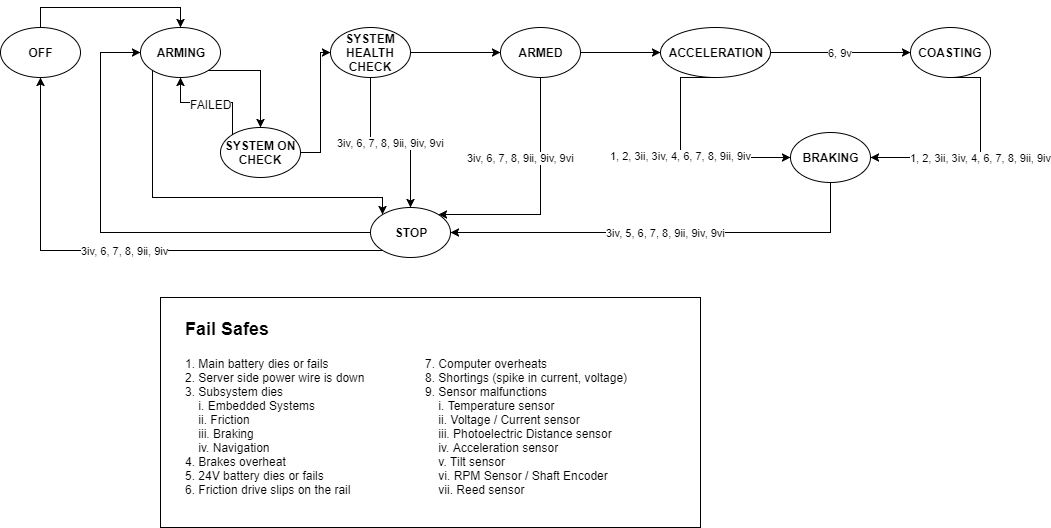
\includegraphics[width=\textwidth]{images/Pod_Failure_Diagram.png}
  \caption{ Pod Failure State Diagram}
  \label{fig:pod-failure-state-diagram}
\end{figure}

    \subsection{Tests \& Validation}
    \begin{itemize}
    \item \textbf{Vacuum Test.} All of the electrical components located on-board of the pod (such as MEB, HPB). While RPIs and ATMega has been tested in a vacuum chamber last year, it is important to test functionality of the entire system, since significant changes have been made. Important points of observation is the machine (RPI and Arduino) and sensor (for a complete sensor list refer to \reffig{tab:pod-sensor-list}) temperature. 
    \item \textbf{Independent Sensor Test.} Validate functionality of all sourced components. Confirm sensor refresh rate and optimal mounting positions.
    \item \textbf{Navigation system test.} Series of HiL tests to simulate pod movement and Unit-test software elements. drive pod without power and measure navigation. Then drive pod with power and measure navigation again
    \item \textbf{Communication System Test.} Stress test entire communication pipeline from sensors to Control-Panel. Goal of test is to find at what network load, the data transfer rate slows down to an unsafe conditions.
    \item \textbf{System / Sub-components Power Loss.} Test complete system power loss scenario as well as partial sub-system power loss.
    \item \textbf{Watchdog reload delay.} Test how long it takes to reload a Master-machine as well as a Hub with OS provided watchdog.
    \end{itemize}


